\section{Cálculos}


\begin{enumerate}
        \item Expresar la ley de velocidad para la reacción.
         Para este caso $ A$ es acetato de etilo y $B$ es el Hidróxido de sodio.

                $$ -r_{a}= k[A][B] $$
        \item Elaborar una gráfica de conductividad en función del tiempo y 
        extrapolar a t = 0.

     \begin{figure}[H]
         \centering
         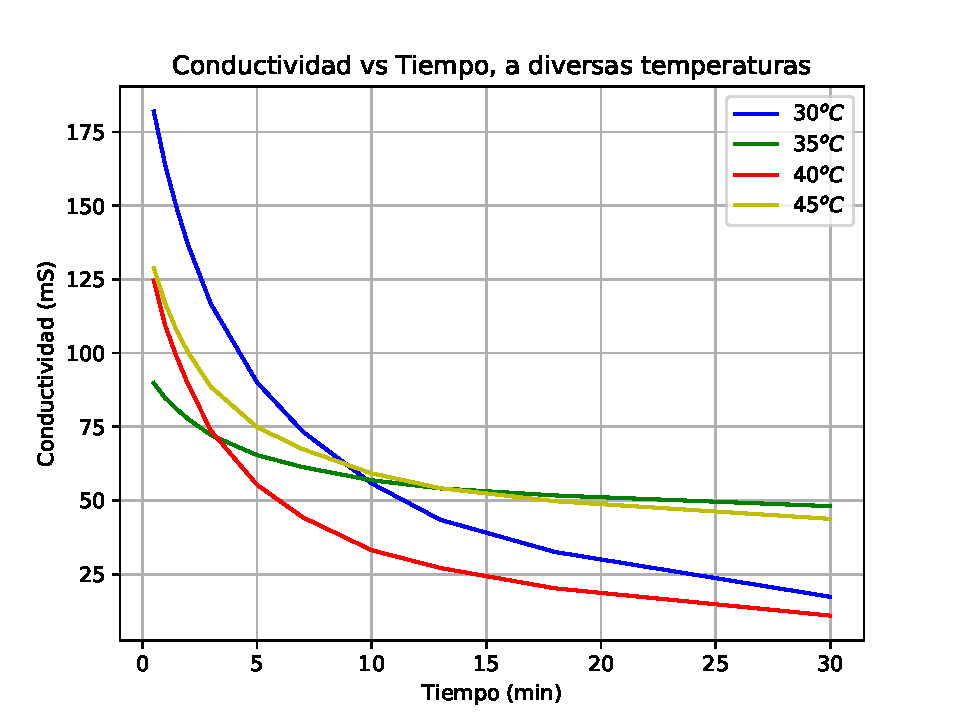
\includegraphics[scale = 0.8]{Figuras/Conductividad_vs_Tiempo.pdf}
         \caption{Diagrama de la pr\'{a}ctica}
      \end{figure}

      \item Plantear las ecuaciones de conductividad en función del tiempo.
       A partir de estas ecuaciones, determinar las concentraciones de los productos 
       que se han formado a cualquier tiempo t, en función de la conductividad.\\
      Con los siguientes  datos se elabora una gráfica de calibración para obtener 
      las concentraciones a cualquier tiempo.

% Table generated by Excel2LaTeX from sheet 'Hoja1'
\begin{table}[H]
  \centering
  \caption{Datos de la práctica}
    \begin{tabular}{crrrr}
    \hline
    \multicolumn{1}{l}{Temperatura} & $30 \: C^{ \circ}$    & $35\: C^{ \circ}$    & $40\: C^{ \circ}$    & $45\: C^{ \circ}$ \\
    \multicolumn{1}{c}{\multirow{2}[0]{*}{Tiempo}} & \multicolumn{1}{p{4.335em}}{Conducti} & \multicolumn{1}{p{4.445em}}{Conducti} & \multicolumn{1}{p{4.28em}}{Conducti} & \multicolumn{1}{p{3.945em}}{Conducti} \\
          & \multicolumn{1}{p{4.335em}}{vidad(mS)} & \multicolumn{1}{p{4.445em}}{vidad(mS)} & \multicolumn{1}{p{4.28em}}{vidad(mS)} & \multicolumn{1}{p{3.945em}}{vidad(mS)} \\ \hline
    0.5   & 181.95 & 89.82 & 124.65 & 128.8 \\
    1     & 163.65 & 84.74 & 109.24 & 116.77 \\
    1.5   & 149.17 & 80.97 & 98.64 & 107.59 \\
    2     & 136.56 & 77.64 & 89.3  & 100.18 \\
    3     & 116.54 & 72.14 & 73.6  & 88.49 \\
    5     & 90.12 & 65.4  & 55.33 & 74.91 \\
    7     & 73.36 & 61.31 & 44.29 & 67.42 \\
    10    & 55.79 & 56.87 & 33.14 & 59.22 \\
    13    & 43.44 & 54.1  & 27.1  & 54.17 \\
    18    & 32.54 & 51.72 & 20.2  & 49.76 \\
    30    & 17.33 & 48.08 & 10.95 & 43.78 \\ \hline
    \end{tabular}%
  \label{tab:addlabel}%
\end{table}%
  

        \begin{figure}[H]
            \centering
            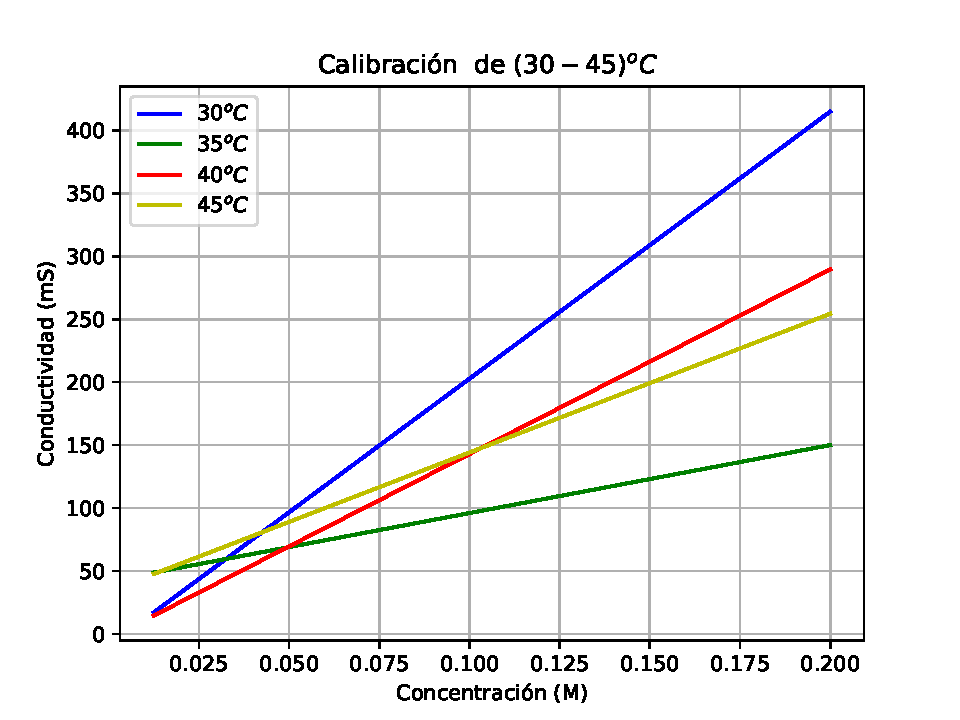
\includegraphics[scale = 0.8]{Figuras/calibracion_todos.pdf}
            \caption{Diagrama de la pr\'{a}ctica}
        \end{figure}

    Con esta gráfica se tiene el ajuste de polinomio:
            $$  Conductividad = m[x] + b$$

        \begin{figure}[H]
            \centering
            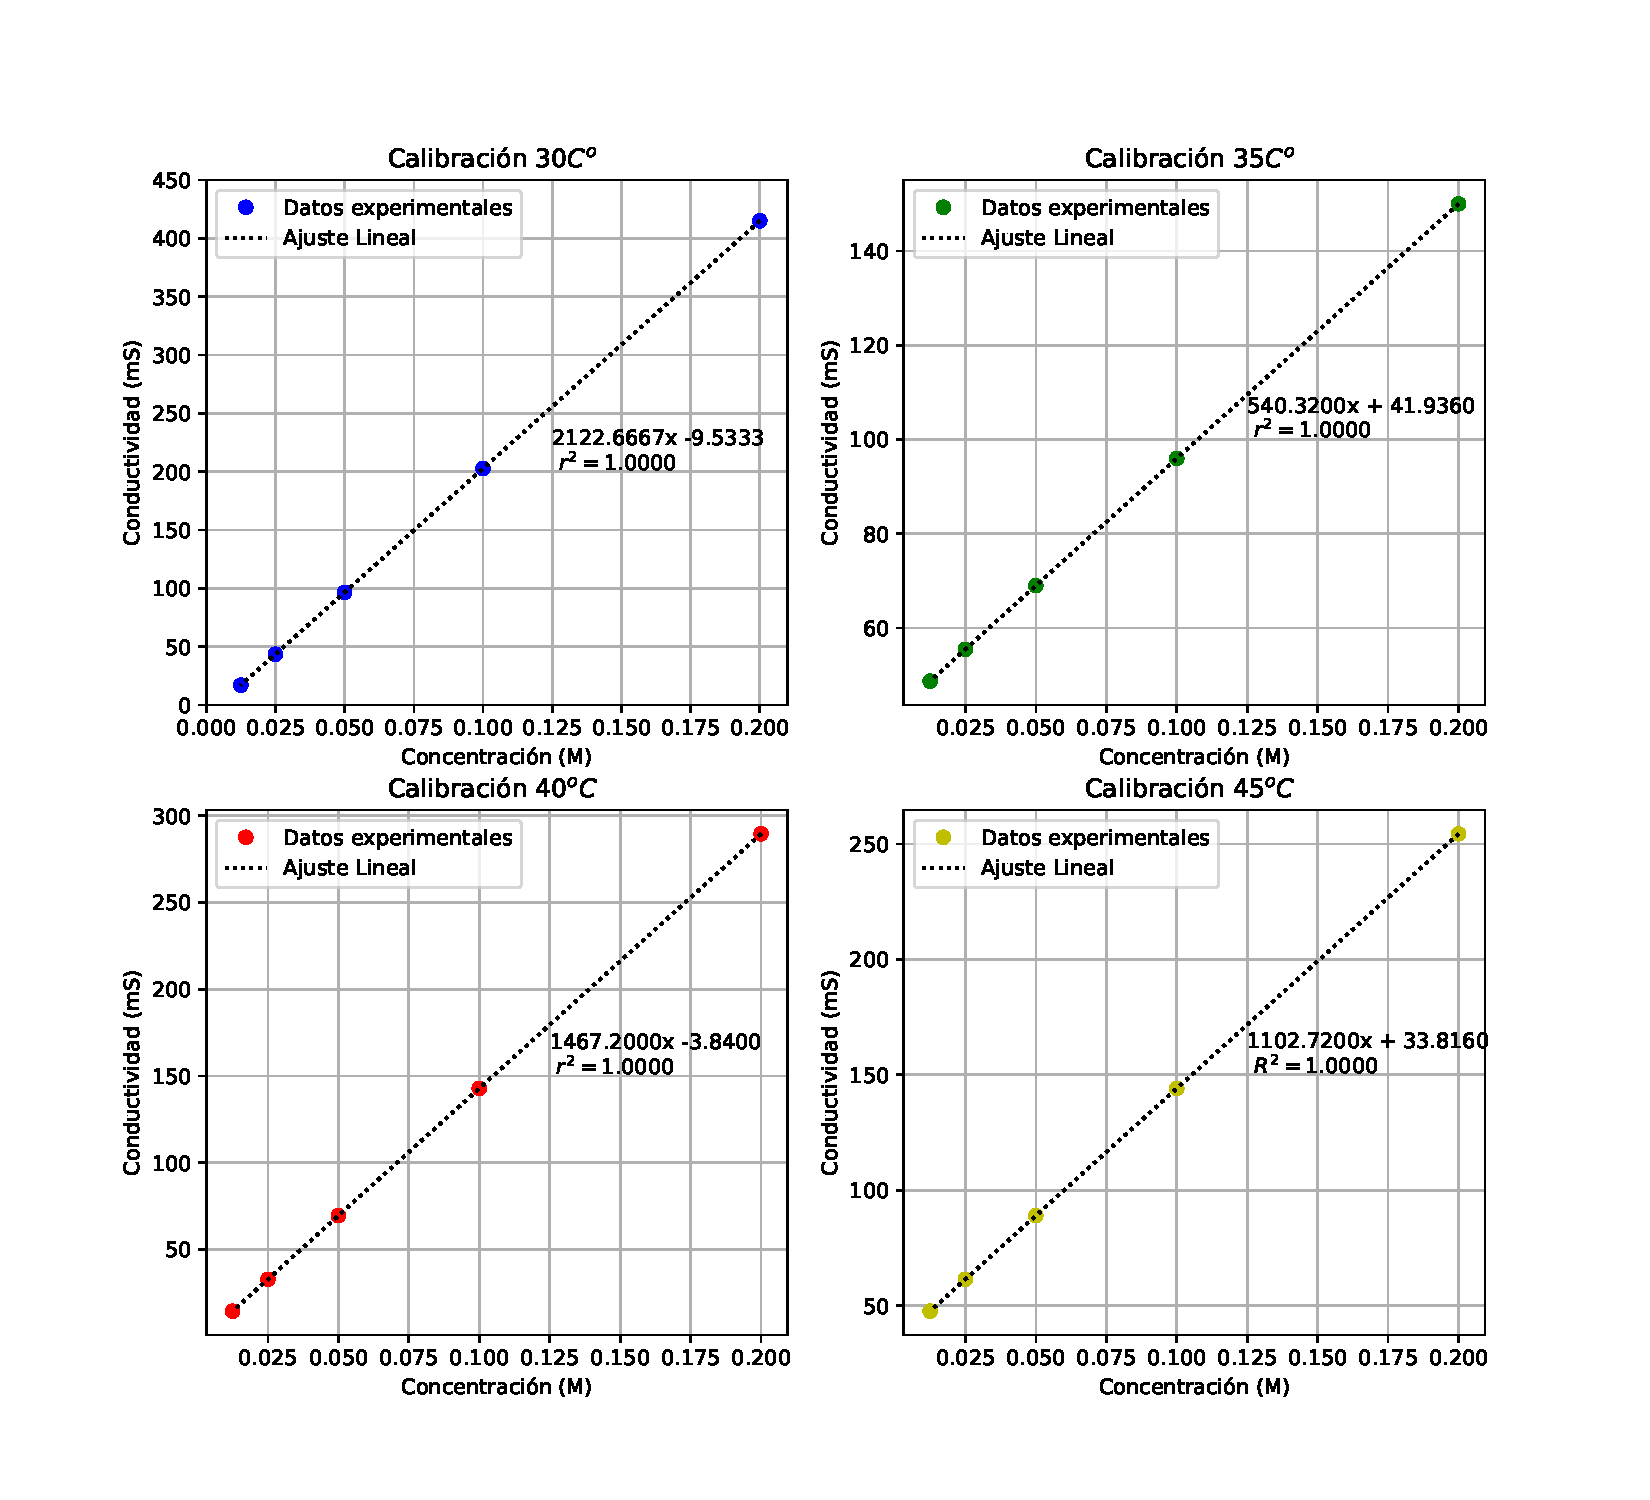
\includegraphics[scale=0.65]{Figuras/FiguraTodos.pdf}
            \caption{Diagrama de la pr\'{a}ctica}
        \end{figure}

\begin{figure}[H]
    \centering
\begin{tabular}{cccc}
\hline
$ T (^{\circ}$C) & Pendiente (m) & Intercepto & $r^{2}$ \\
\hline
30 & 2122.7 & -9.5334  & 1   \\
35 & 540.32 & +41.936  & 1   \\
40 & 1467.2 & -3.84    & 1   \\
45 & 1102.7 & +33.813  & 1   \\
\hline

\end{tabular} 
\caption{Datos  de calibración }
    \label{fig:my_label}
\end{figure}


    Despejando para la concentración tenemos que:
            $$ [x]= \dfrac{Conductividad + b}{m}$$
            
    Se calculan las concentraciones siguientes:\\

\begin{table}[H]
    \centering
    \begin{tabular}{crrrr}
        \hline
        
        \multicolumn{1}{l}{Temperatura} & $30 C^{\circ} $   & $35 \: C^{\circ}$    & $40 \: C^{\circ}$    & $45 \: C^{\circ}$ \\ \hline
        \multicolumn{1}{c}{\multirow{2}[0]{*}{Tiempo}} & \multicolumn{1}{p{5.39em}}{Concen-} & \multicolumn{1}{p{5.39em}}{Concen-} & \multicolumn{1}{p{5.39em}}{Concen-} & \multicolumn{1}{p{5.39em}}{Concen-} \\ 
              & \multicolumn{1}{p{5.39em}}{tración (M)} & \multicolumn{1}{p{5.39em}}{tración (M)} & \multicolumn{1}{p{5.39em}}{tración (M)} & \multicolumn{1}{p{5.39em}}{tración (M)} \\ \hline
        0.5   & 0.09021 & 0.08862 & 0.08757 & 0.08614 \\
        1     & 0.08159 & 0.07922 & 0.07707 & 0.07523 \\
        1.5   & 0.07476 & 0.07224 & 0.06985 & 0.0669  \\
        2     & 0.06882 & 0.06608 & 0.06348 & 0.06018 \\
        3     & 0.05939 & 0.0559  & 0.05278 & 0.04958 \\
        5     & 0.04695 & 0.04343 & 0.04033 & 0.03727 \\
        7     & 0.03905 & 0.03586 & 0.0328  & 0.03047 \\
        10    & 0.03077 & 0.02764 & 0.0252  & 0.02304 \\
        13    & 0.02496 & 0.02251 & 0.02109 & 0.01846 \\
        18    & 0.01982 & 0.01811 & 0.01638 & 0.01446 \\
        30    & 0.01266 & 0.01137 & 0.01008 & 0.00904 \\ 
        
        \hline
    \end{tabular}
    \caption{Tabla de concentraciones a diferentes temperaturas}
    \label{tab:concentracion}
\end{table}
  

    \item Utilizando las concentraciones anteriormente calculadas, determinar el orden de
    reacción y la constante de velocidad por el método integral gráfico.\\
    Para calcular el orden de reacción se gráfica $t$ vs $1/C_a$\\

\begin{table}[H]
    \centering
    \begin{tabular}{crrrr}
        \hline

        \multicolumn{1}{l}{Temperatura} & $30\: ^{\circ} C$    & $35\: ^{\circ} C$    & $40\: ^{\circ} C$    & $45\: ^{\circ} C$ \\ \hline 
        \multicolumn{1}{c}{\multirow{2}[0]{*}{Tiempo}} & \multicolumn{1}{p{4.5em}}{$1/Ca$} & \multicolumn{1}{p{5.78em}}{$1/Ca$} & \multicolumn{1}{p{6em}}{$1/Ca$} & \multicolumn{1}{p{5.39em}}{$1/Ca$} \\ 
              &       &       &       &  \\ \hline
        0.5   & 11.08556 & 11.28394 & 11.41879 & 11.60932 \\
        1     & 12.25695 & 12.62312 & 12.97489 & 13.29291 \\
        1.5   & 13.37526 & 13.84229 & 14.31694 & 14.94700 \\
        2     & 14.52975 & 15.13332 & 15.75263 & 16.61594 \\
        3     & 16.83702 & 17.88902 & 18.94628 & 20.16864 \\
        5     & 21.30083 & 23.02762 & 24.79635 & 26.83360 \\
        7     & 25.60759 & 27.88892 & 30.48411 & 32.81455 \\
        10    & 32.49525 & 36.18053 & 39.67550 & 43.40655 \\
        13    & 40.07105 & 44.4196  & 47.42081 & 54.17608 \\
        18    & 50.4523  & 55.22486 & 61.03161 & 69.16081 \\
        30    & 79.01829 & 87.94271 & 99.20216 & 110.6684 \\ 
        \hline
        
        \end{tabular}
    \caption{Inversa de la concentración a las diferentes temperaturas}
    \label{tab:inversa_concentracion}
  \end{table}%
  

    \begin{figure}[H]
        \centering
        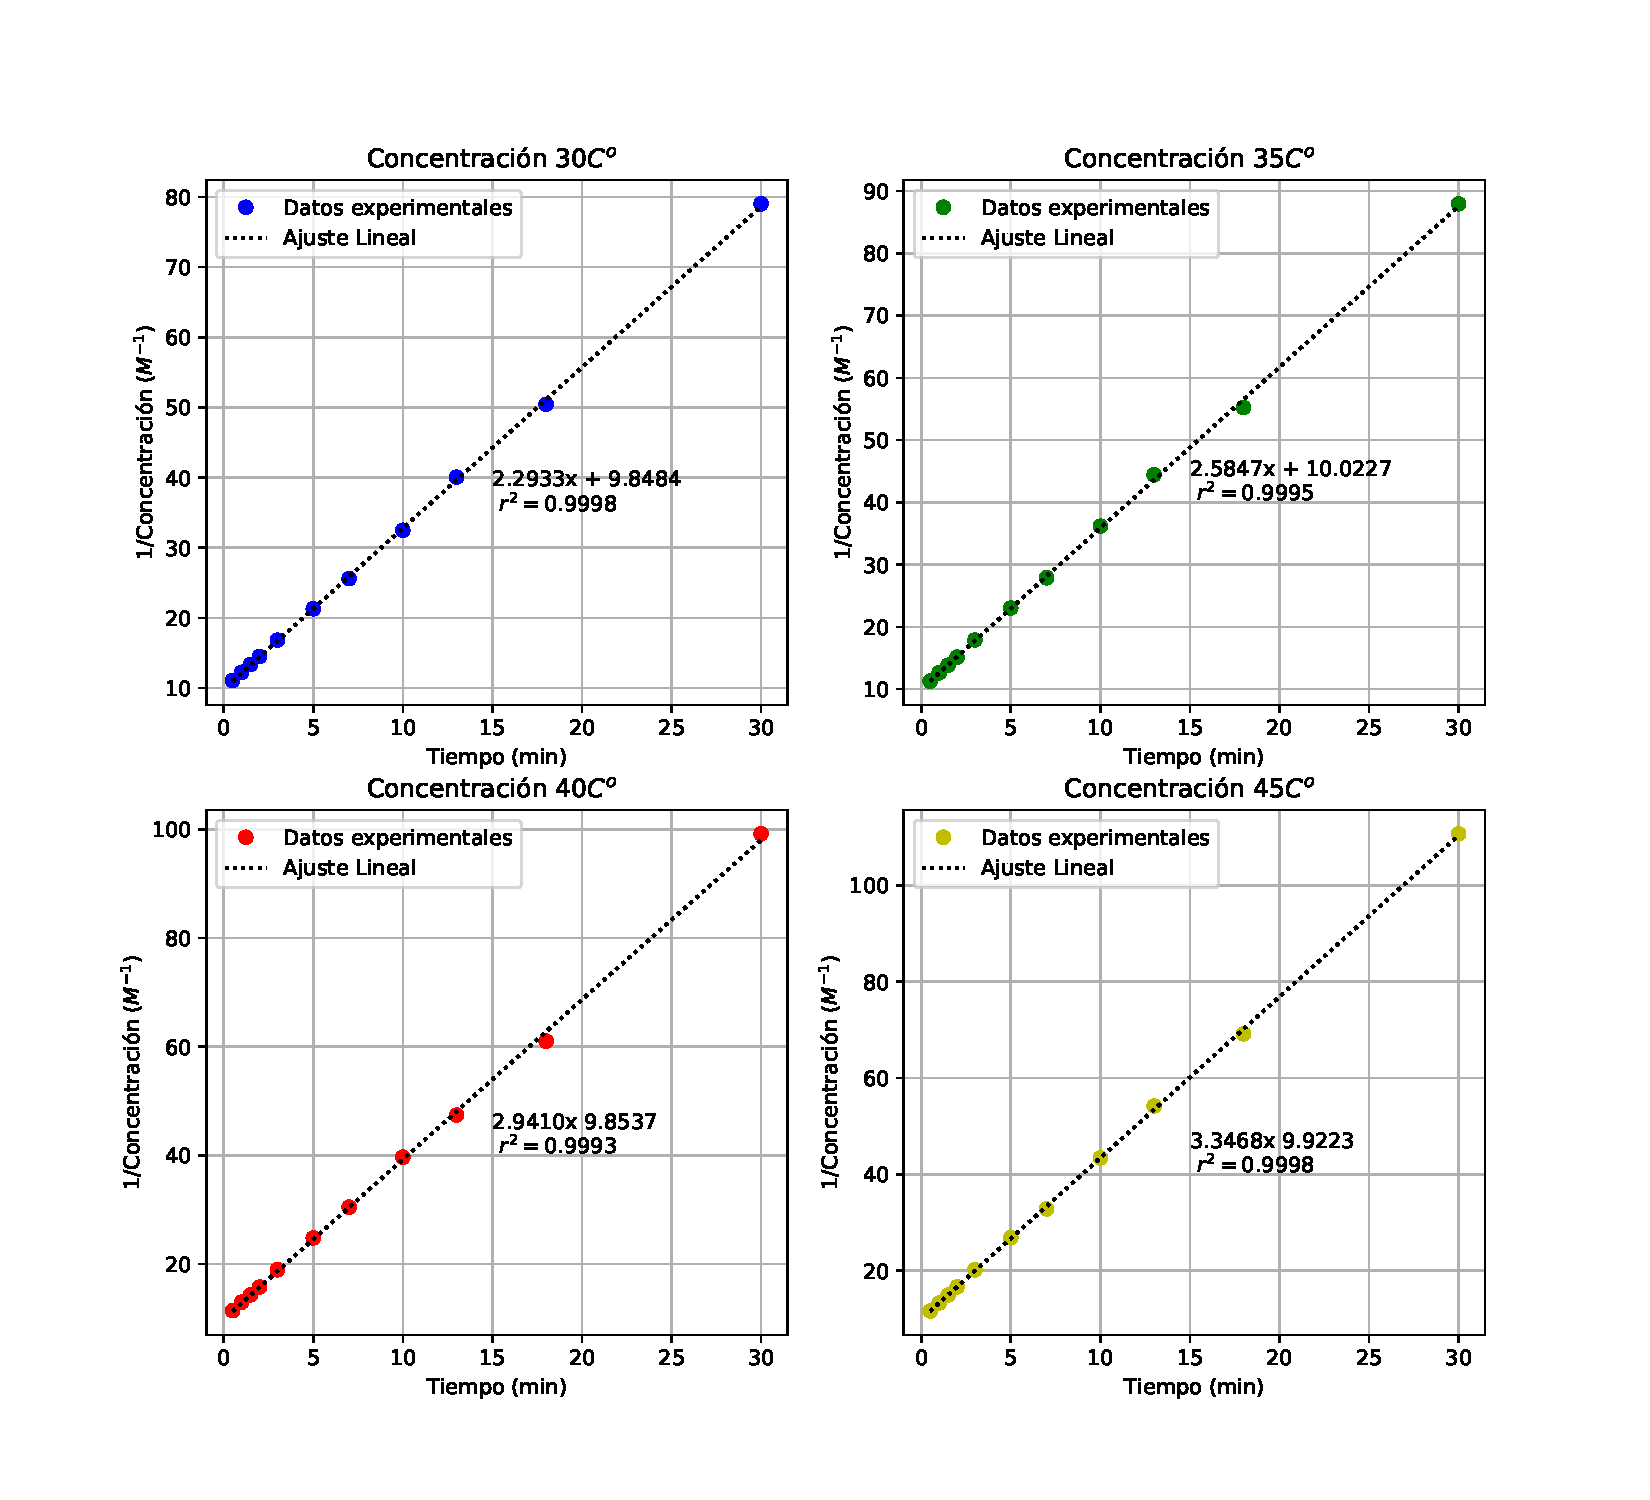
\includegraphics[scale=0.65]{Figuras/Ctodos.pdf}
        \caption{Diagrama de la pr\'{a}ctica}
    \end{figure}

    \begin{figure}[H]
        \centering
        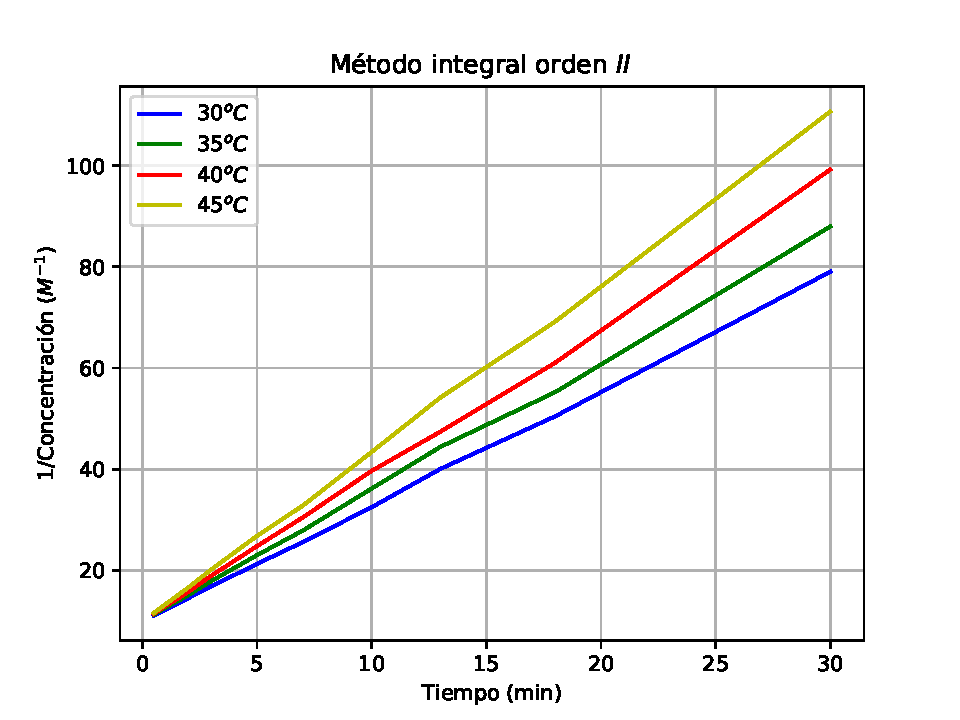
\includegraphics[scale = 0.8]{Figuras/concentracion_todos.pdf}
        \caption{Diagrama de la pr\'{a}ctica}
    \end{figure}



\begin{figure}[H]
    \centering
    \begin{tabular}{cccc}
    \hline
    $ T (^{\circ}$C) & Pendiente(m)=$k$  & Intercepto & $r^{2}$ \\
    \hline
    30 & 2.2934 & 9.8485   & 0.9998  \\
    35 & 2.5847 & 10.023   & 0.9995   \\
    40 & 2.9410 & 9.8537   & 0.9993   \\
    45 & 3.3467 & 9.9221   & 0.9998   \\
    \hline

    \end{tabular} 
\caption{Constantes a diferentes $T$}
    \label{fig:my_label}
\end{figure}\\

    Recordemos que la pendiente  es la contante cinética $ k $, por  el valor de $ r^{2}$  podemos decir que la reacción es de \textbf{orden II}
    \item Calcular el factor de frecuencia (A) y la energía de activación (Ea).\\
    Para calcular los parámetros es necesario tomar las constantes y las temperaturas
    anteriores, aplicando $ln(k)$   y la inversa de la temperatura. Se obtuvo los 
    siguientes datos:\\

\begin{figure}[H]
    \centering
    \begin{tabular}{cccc}
    \hline
    $T$ K & $k$  & $1/T$ & $Ln(k)$ \\
    \hline
    303	& 2.2934 &	0.0033	& 0.8300 \\
    308	& 2.5847 &	0.0032	& 0.9496 \\
    313	& 2.9410 &	0.0032	& 1.0787 \\
    318	& 3.3467 &	0.0031	& 1.2080 \\

    \hline

    \end{tabular} 
\caption{Datos para ecuación de Arrhenius}
    \label{fig:my_label}
\end{figure}\\

Para determinar el parámetro $A$  tenemos que el intercepto $b= 8.8544 = ln(A) $ , despejando tenemos que $A= 7005.144$. Para determinar la energia de activación tenemos que $m= -E_{a}/R$
despejando  tenemos que $E_{a}= 20227.030 J/mol*K$

    \begin{figure}[H]
        \centering
        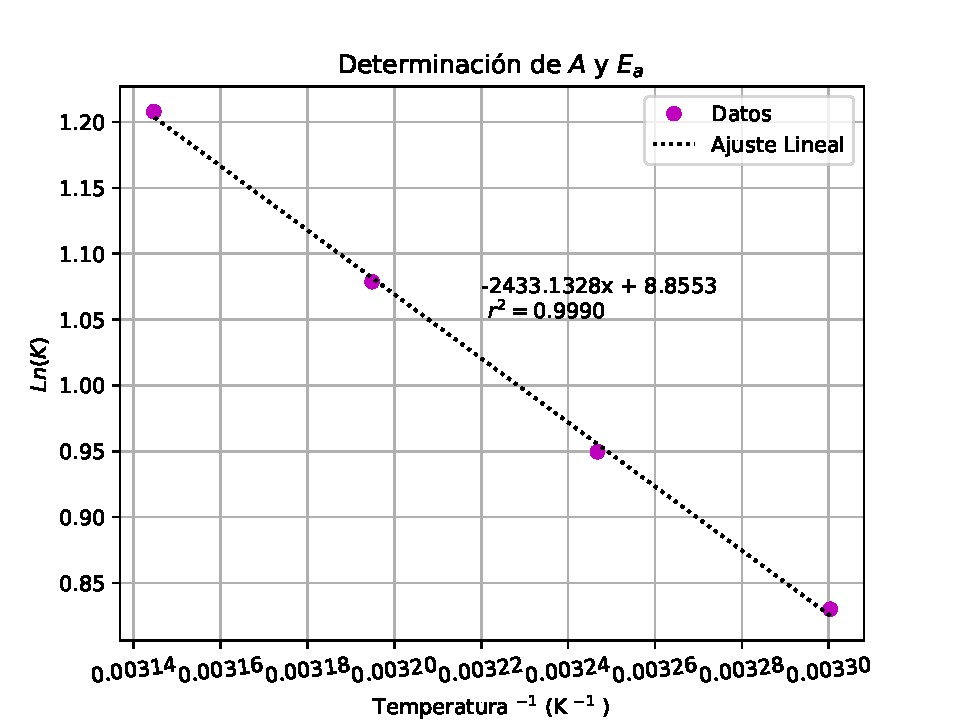
\includegraphics[scale = 0.8]{Figuras/ln_k_t.pdf}
        \caption{Diagrama de la pr\'{a}ctica}
    \end{figure}


\end{enumerate}
